%--------------------------------------------------------------
% moneyLaundering.tex (use thesis.tex as main file)
%--------------------------------------------------------------
\chapter{Financial Crime and Money Laundering}
\label{moneyLaundering}
%--------------------------------------------------------------
Understanding how money laundering works is fundamental to garantee both an effective and explainable detection of suspicious transaction. 
This chapter offers a theoretical introduction to money laundering providing a mathematical formulation of the problem together with a summary of common strategies employed by criminals to avoid detection.
\section{The Limitations of the Lonely Scammer}
Individual scammers typically rely on simple and intuitive techniques to introduce illicit funds into the legitimate economy. One of the most prevalent methods is known as ``smurfing''. In simple terms, smurfing involves breaking down a large sum of illicit money into many smaller, inconspicuous chunks to deposit them without raising suspicion. 

More formally, individual scammers rely on smurfing to avoid Anti-Money Laundering (AML) detection mechanisms, which usually flag transactions above a specific threshold $\tilde{x}$. By splitting their initial illicit funds $x$ into smaller transactions $x_n$, such that each transaction satisfies $x_n \leq \tilde{x}$, they minimize the risk of detection \cite{contreras2026strategic}. The mathematical expectation of profit $\pi_s$ for a scammer engaging in smurfing can be defined as:
\begin{equation}
    \pi_s = x(1-\nu)
\end{equation}
where $x$ represents the total initial illicit funds, and $\nu \in (0,1)$ is the friction cost or commission proportion associated with the smurfing process (e.g., the fee paid to mules). 

While smurfing is effective for small amounts, its scalability is severely limited. When attempting to launder much larger volumes of funds, an individual scammer operating from a single account faces a significantly higher probability of detection $(1-p)$, where $p$ is the probability of successfully avoiding detection. If caught, the scammer is subjected to a severe monetary penalty $T$, which includes both the total confiscation of the funds and associated judicial fines \cite{contreras2026strategic}. Therefore, operating as a ``lonely scammer'' becomes mathematically and practically unviable for large-scale operations due to the massive expected cost of $(1-p)T$.

\section{Fraud Rings}
In regard to overcome those issues, criminals have improved their techniques by employing highly sophisticated obfuscation tactics. Instead of acting alone, they form complex ``fraud rings'' to distribute illicit funds across vast networks of temporary accounts. To further break the traceable link between sender and receiver, illicit actors frequently use cyclic transfers and cryptocurrency \textbf{mixers} services that pool together funds from multiple users, mix them, and redistribute them at random intervals and amounts. These advanced tactics create dense, highly camouflaged transaction topologies that easily evade threshold-based rules and simple heuristic detection methods.

To achive their goal they utilize a strategy of transaction layering, often characterized by a topological depth $L$, and network diversification to obscure the money trail \cite{contreras2026strategic, li2025scamsweeper}.
By spreading the funds through a complex topology, the fraud ring successfully increases its non-detection probability $p_L$, which now depends explicitly on the layering depth $L$. The expected profit of a fraud ring utilizing $L$ layers can be mathematically expressed as:
\begin{equation}
    E[\pi_L] = p_L x - (1-p_L)T - c(L)
\end{equation}
where $E[\pi_L]$ is the expected profit, $p_L$ is the enhanced probability of evading detection when $L$ layers are used, $x$ is the total illicit funds, $T$ is the total penalty if caught, and $c(L)$ represents the monotonic cost function associated with establishing and maintaining the $L$ transaction layers. Because the fraud ring dramatically increases the probability of evading detection ($p_L \to 1$ as $L$ increases), the expected payoff remains highly profitable even when factoring in the complex layering costs $c(L)$ \cite{contreras2026strategic}. 

\section{Money Laundering patterns}
Understanding the structural patterns that criminality assumes is fundamental to develop effective detection models and to employ strategies to enhance the explainability of them. According to the literature, there are 8 different patterns that are often used in ML \cite{AMLSim, AMLWorld}. 
\begin{figure}
    \centering
    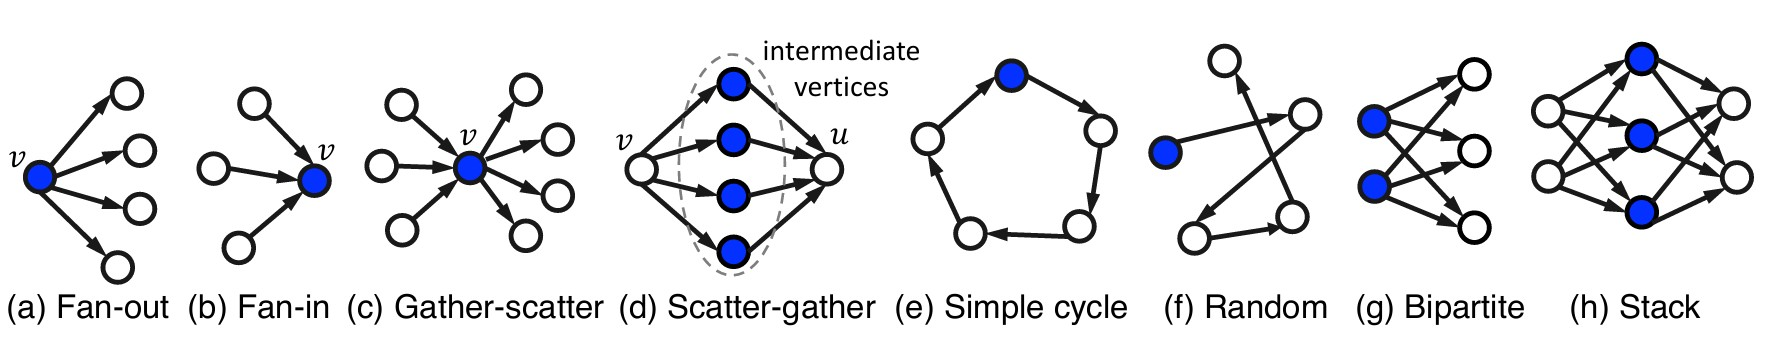
\includegraphics[width=1\textwidth]{IMG/laundering_patterns.jpg}
    \caption{Money Laundering patterns}
    \label{fig:launderingPatterns}
\end{figure}
Which are: 
\begin{itemize}
    \item \textit{fan-out}, shown in Figure \ref{fig:launderingPatterns} a, characterized by outgoing edges from a node $v$ to more than 2 adjacent nodes; 
    \item \textit{fan-in}, Figure \ref{fig:launderingPatterns} b, $v$ is connected to more than 2 nodes by incoming edges;
    \item \textit{gather-scatter}, Figure \ref{fig:launderingPatterns} c, is the combination of a fan-in and a fan-out pattern on the same node $v$;
    \item \textit{scatter-gather}, Figure \ref{fig:launderingPatterns} d, also composed by a fan-in and a fan-out pattern but on two different nodes, sharing the same intermediate neighbors;
    \item \textit{simple-cycle}, Figure \ref{fig:launderingPatterns} e, characterized by a sequence of transactions that starts and ends at the same node;
    \item \textit{random}, Figure \ref{fig:launderingPatterns} f, similar to the cycle but founds do not return to the original account;
    \item \textit{bipartite}, Figure \ref{fig:launderingPatterns} g, moves founds from a set of original nodes to a set of target nodes, with no transactions between accounts of the same set;
    \item \textit{stack}, Figure \ref{fig:launderingPatterns} h, extends the bipartite pattern by adding a second bipartite layer.
\end{itemize}
It's important to mention that in some cases some patterns can be found in both illicit and licit transactions \cite{AMLgentex}. Specifically, \textit{fan-in} and \textit{fan-out} are patterns that are also frequent in legitimate, every-day transactions, such as salary payments or transfers between family members or friends.
That being said, the detection of such patterns remains a foundamental component of any money laundering detection models, albeit insufficient on its own.
Furthermore, a model that correctly classifies those patterns provides a much more interpretable result than one that simply performs a binary classification between licit and illicit transactions. In Chapter \ref{ethics_privacy_regulations} we will see why explainability is of fundamental importance in the financial field. 

